\documentclass[a4paper]{article}
\usepackage{times}
\usepackage[utf8]{inputenc}
\usepackage{selinput}
\usepackage{upquote}
\usepackage[margin=2cm, rmargin=4cm, tmargin=3cm]{geometry}
\usepackage{tcolorbox}
\usepackage{xspace}
\usepackage[french]{babel}
\usepackage{url}
\usepackage{hyperref}
\usepackage{fontawesome5}
\usepackage{marginnote}
\usepackage{ulem}
\usepackage{tcolorbox}
\usepackage{graphicx}
%\usepackage[top=Bcm, bottom=Hcm, outer=Ccm, inner=Acm, heightrounded, marginparwidth=Ecm, marginparsep=Dcm]{geometry}


\newtcolorbox{Example}[1]{colback=white,left=20pt,colframe=slideblue,fonttitle=\bfseries,title=#1}
\newtcolorbox{Solutions}[1]{colback=white,left=20pt,colframe=green,fonttitle=\bfseries,title=#1}
\newtcolorbox{Conseils}[1]{colback=white,left=20pt,colframe=slideblue,fonttitle=\bfseries,title=#1}
\newtcolorbox{Warning}[1]{colback=white,left=20pt,colframe=warning,fonttitle=\bfseries,title=#1}

\setlength\parindent{0pt}

  %Exercice environment
  \newcounter{exercice}
  \newenvironment{Exercice}[1][]
  {
  \par
  \stepcounter{exercice}\textbf{Question \arabic{exercice}:} (\faClock \enskip \textit{#1})
  }
  {\bigskip}
  

% Title
\newcommand{\titre}{\begin{center}
  \section*{Algorithmes et Pensée Computationnelle}
\end{center}}
\newcommand{\cours}[1]
{\begin{center} 
  \textit{#1}\\
\end{center}
  }


\newcommand{\exemple}[1]{\newline~\textbf{Exemple :} #1}
%\newcommand{\attention}[1]{\newline\faExclamationTriangle~\textbf{Attention :} #1}

% Documentation url (escape \# in the TP document)
\newcommand{\documentation}[1]{\faBookOpen~Documentation : \href{#1}{#1}}

% Clef API
\newcommand{\apikey}[1]{\faKey~Clé API : \lstinline{#1}}
\newcommand{\apiendpoint}[1]{\faGlobe~Url de base de l'API \href{#1}{#1}}

%Listing Python style
\usepackage{color}
\definecolor{slideblue}{RGB}{33,131,189}
\definecolor{green}{RGB}{0,190,100}
\definecolor{blue}{RGB}{121,142,213}
\definecolor{grey}{RGB}{120,120,120}
\definecolor{warning}{RGB}{235,186,1}

\usepackage{listings}
\lstdefinelanguage{texte}{
    keywordstyle=\color{black},
    numbers=none,
    frame=none,
    literate=
           {é}{{\'e}}1
           {è}{{\`e}}1
           {ê}{{\^e}}1
           {à}{{\`a}}1
           {â}{{\^a}}1
           {ù}{{\`u}}1
           {ü}{{\"u}}1
           {î}{{\^i}}1
           {ï}{{\"i}}1
           {ë}{{\"e}}1
           {Ç}{{\,C}}1
           {ç}{{\,c}}1,
    columns=fullflexible,keepspaces,
	breaklines=true,
	breakatwhitespace=true,
}
\lstset{
    language=Python,
	basicstyle=\bfseries\footnotesize,
	breaklines=true,
	breakatwhitespace=true,
	commentstyle=\color{grey},
	stringstyle=\color{slideblue},
  keywordstyle=\color{slideblue},
	morekeywords={with, as, True, False, Float, join, None, main, argparse, self, sort, __eq__, __add__, __ne__, __radd__, __del__, __ge__, __gt__, split, os, endswith, is_file, scandir, @classmethod},
	deletekeywords={id},
	showspaces=false,
	showstringspaces=false,
	columns=fullflexible,keepspaces,
	literate=
           {é}{{\'e}}1
           {è}{{\`e}}1
           {ê}{{\^e}}1
           {à}{{\`a}}1
           {â}{{\^a}}1
           {ù}{{\`u}}1
           {ü}{{\"u}}1
           {î}{{\^i}}1
           {ï}{{\"i}}1
           {ë}{{\"e}}1
           {Ç}{{\,C}}1
           {ç}{{\,c}}1,
    numbers=left,
}

\newtcbox{\mybox}{nobeforeafter,colframe=white,colback=slideblue,boxrule=0.5pt,arc=1.5pt, boxsep=0pt,left=2pt,right=2pt,top=2pt,bottom=2pt,tcbox raise base}
\newcommand{\projet}{\mybox{\textcolor{white}{\small projet}}\xspace}
\newcommand{\optionnel}{\mybox{\textcolor{white}{\small Optionnel}}\xspace}
\newcommand{\advanced}{\mybox{\textcolor{white}{\small Pour aller plus loin}}\xspace}
\newcommand{\auto}{\mybox{\textcolor{white}{\small Auto-évaluation}}\xspace}


\usepackage{environ}
\newif\ifShowSolution
\NewEnviron{solution}{
  \ifShowSolution
	\begin{Solutions}{\faTerminal \enskip Solution}
		\BODY
	\end{Solutions}
  \fi}


  \usepackage{environ}
  \newif\ifShowConseil
  \NewEnviron{conseil}{
    \ifShowConseil
    \begin{Conseils}{\faLightbulb \quad Conseil}
      \BODY
    \end{Conseils}

    \fi}

    \usepackage{environ}
  \newif\ifShowWarning
  \NewEnviron{attention}{
    \ifShowWarning
    \begin{Warning}{\faExclamationTriangle \quad Attention}
      \BODY
    \end{Warning}

    \fi}
  

%\newcommand{\Conseil}[1]{\ifShowIndice\ \newline\faLightbulb[regular]~#1\fi}



\usepackage{array}
\newcolumntype{C}[1]{>{\centering\let\newline\\\arraybackslash\hspace{0pt}}m{#1}}

\begin{document}

% Change the following values to true to show the solutions or/and the hints
\ShowSolutiontrue
\ShowConseiltrue
\titre
\cours{Architecture des ordinateurs}

Le but de cette séance est de comprendre le fonctionnement d'un ordinateur. La série d'exercices sera axée autour de de conversions en base binaire, décimale ou hexadécimal, de calcul de base en suivant le modèle Von Neumann. \\

\section{Conversions}

\begin{Exercice}[5 minutes]  \textbf{Conversion $Base_{10}$ - $Base_2$}\\
    \begin{enumerate}
        \item Convertir le nombre 10$_{(10)}$ en base 2.
        \item Convertir le nombre 45$_{(10)}$ en base 2.
        \item Convertir le nombre 173$_{(10)}$ en base 2.
    \end{enumerate}

    \begin{conseil}
        TODO: Conseils pour passer de la base décimale à la base binaire \\
        Useful link: http://www.circuits-logiques.polymtl.ca/help/Chapitre05.pdf
    \end{conseil}
    \begin{solution}
        Présenter les étapes détaillées permettant d'aboutir à la solution.
    \end{solution}
\end{Exercice}


\begin{Exercice}[15 minutes]  \textbf{Conversion $Base_{10}$ - $Base_3$, $Base_8$, $Base_{16}$}\\
    \begin{enumerate}
        \item Convertir le nombre 40$_{(10)}$ en base 8.
        \item Convertir le nombre 52$_{(10)}$ en base 3.
        \item Convertir le nombre 254$_{(10)}$ en base 16.
    \end{enumerate}

    \begin{conseil}
        TODO: Conseils pour passer de la base décimale aux bases 3, 8 et 16.
    \end{conseil}
    \begin{solution}
        Présenter les étapes détaillées permettant d'aboutir à la solution.
    \end{solution}
\end{Exercice}

\begin{Exercice}[15 minutes] \textbf{Conversion $Base_{3}$ - $Base_{16}$ en $Base_8$}
    \begin{enumerate}
        \item Convertir le nombre 10110$_{(2)}$ en base 10.
        \item Convertir le nombre 4321$_{(5)}$ en base 10.
        \item Convertir le nombre ABC$_{(16)}$ en base 10.
    \end{enumerate}
    \begin{conseil}
        TODO: Conseils pour passer des bases 3 et 16 à la base 10.
    \end{conseil}
    \begin{solution}
        Présenter les étapes détaillées permettant d'aboutir à la solution.
    \end{solution}

\end{Exercice}
\newpage

\section{Arithmétique binaire}

\begin{Exercice}[15 minutes] \textbf{Addition de nombres binaires}
    \begin{enumerate}
        \item Additionner \lstinline{01010101}$_{(2)}$ et \lstinline{10101010}$_{(2)}$
        \item Additionner \lstinline{01011111}$_{(2)}$ et \lstinline{10000001}$_{(2)}$
        \item Additionner \lstinline{01110100}$_{(2)}$ et \lstinline{00011010}$_{(2)}$
    \end{enumerate}
    \begin{conseil}
\textbf{Table d'addition binaire:}\\
        \begin{tabular}{| C{0.1\textwidth} | C{0.1\textwidth} | C{0.1\textwidth} | C{0.1\textwidth} |} 
            \hline
            \textbf{a} & \textbf{b} & \textbf{s=a+b} & \textbf{r}\\ [0.5ex]
            \hline
            0 & 0 & 0 & 0 \\ [0.5ex] 
            \hline
            0 & 1 & 1 & 0 \\ [0.5ex] 
            \hline
            1 & 0 & 1 & 0 \\ [0.5ex] 
            \hline
            1 & 1 & 0 & 1 \\ [0.5ex] 
            \hline
        \end{tabular}
    \end{conseil}
    TODO: Rajouter un exemple
    \begin{solution}
        Présenter les étapes détaillées permettant d'aboutir à la solution.
    \end{solution}
\end{Exercice}

\begin{Exercice}[15 minutes] \textbf{Soustraction de nombres binaires}\\
    Effectuer les opérations suivantes:

    \begin{enumerate}
        \item 01111111$_{(2)}$ - 01000000$_{(2)}$
        \item 10000000$_{(2)}$ - 00000001$_{(2)}$
        \item 10101010$_{(2)}$ - 01010101$_{(2)}$
    \end{enumerate}

    \begin{conseil}
        \textbf{Table de soustraction binaire:}\\
        \begin{tabular}{| C{0.1\textwidth} | C{0.1\textwidth} | C{0.1\textwidth} | C{0.1\textwidth} |} 
            \hline
            \textbf{a} & \textbf{b} & \textbf{s=a-b} & \textbf{r}\\ [0.5ex]
            \hline
            0 & 0 & 0 & 0 \\ [0.5ex] 
            \hline
            0 & 1 & 1 & 1 \\ [0.5ex] 
            \hline
            1 & 0 & 1 & 0 \\ [0.5ex] 
            \hline
            1 & 1 & 0 & 0 \\ [0.5ex] 
            \hline
        \end{tabular}
    \end{conseil}
    TODO: Rajouter un exemple
    \begin{solution}
        Présenter les étapes détaillées permettant d'aboutir à la solution.
    \end{solution}

    \textbf{\\ \faTerminal  Exemple:}
        \begin{figure}[h]
            \centering
            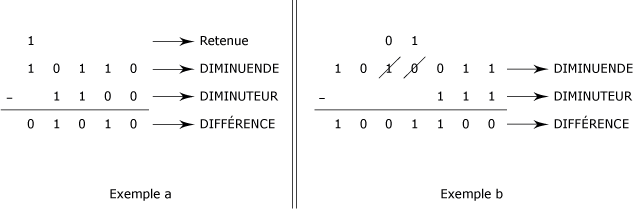
\includegraphics[width=0.52\textwidth]{img/substract.png}
            \caption{Exemple de soustraction de nombres binaires}
        \end{figure}

\end{Exercice}
\newpage
\section{Conversion et arithmétique}
\begin{Exercice}[20 minutes] \textbf{Conversion et addition:}\\
    Effectuer les opérations suivantes:
    \begin{enumerate}
        \item 111101$_{(2)}$ + 110$_{(2)}$ = ...$_{(10)}$
        \item 111111$_{(2)}$ + 000001$_{(2)}$ = ...$_{(10)}$
        \item 127$_{(10)}$ + ABC$_{(16)}$ = ...$_{(8)}$
    \end{enumerate}
    \begin{conseil}
        TODO: Conseils pour convertir puis additionner des nombres de bases différentes.
    \end{conseil}
    \begin{solution}
        Présenter les étapes détaillées permettant d'aboutir à la solution.
    \end{solution}
\end{Exercice}

\begin{Exercice}[20 minutes] \textbf{Conversion et soustraction:}\\
    Effectuer les opérations suivantes:
    \begin{enumerate}
        \item 101010$_{(2)}$ - 010101$_{(2)}$ = ...$_{(10)}$
        \item 64$_{(10)}$ - 001000$_{(2)}$ = ...$_{(10)}$
        \item FFF$_{(10)}$ - 127$_{(10)}$ = ...$_{(2)}$
    \end{enumerate}
    \begin{conseil}
        TODO: Conseils pour convertir puis soustraire des nombres de bases différentes.
    \end{conseil}
    \begin{solution}
        Présenter les étapes détaillées permettant d'aboutir à la solution.
    \end{solution}
\end{Exercice}


\newpage
\section{Modèle de Von Neuman}
Dans cette section, nous allons simuler une opération d'addition dans le \textbf{modèle de Van Neumann}, il va vous être demandé à chaque étape (FDES) de donner la valeur des registres.\\

\textbf{État d'origine:}\\
A l'origine, notre \lstinline{Process Counter (PC)} vaut \lstinline{00100000}.\\

Dans la mémoire, les instructions sont les suivantes:

\begin{tabular}{| C{0.1\textwidth} | C{0.1\textwidth} |} 
    \hline
    \textbf{Adresse} & \textbf{Valeur}\\ [0.5ex]
    \hline
    00011111 & 00100100\\ [0.5ex] 
    \hline
    00100000 & 10110110\\ [0.5ex] 
    \hline
    00100001 & 11101101\\ [0.5ex]
    \hline
\end{tabular}
\\\\
Les registres sont les suivantes:

\begin{tabular}{| C{0.1\textwidth} | C{0.1\textwidth} |} 
    \hline
    \textbf{Registre} & \textbf{Valeur}\\ [0.5ex]
    \hline
    00 & 11100011\\ [0.5ex] 
    \hline
    01 & 01101100\\ [0.5ex] 
    \hline
    10 & 00100101\\ [0.5ex] 
    \hline
    11 & 00000000\\ [0.5ex]
    \hline
\end{tabular}
\\\\
Les opérations disponibles pour l'unité de contrôle sont les suivantes:
\\
\begin{tabular}{| C{0.1\textwidth} | C{0.1\textwidth} |} 
    \hline
    \textbf{Numéro} & \textbf{Valeur}\\ [0.5ex]
    \hline
    00 & MOV\\ [0.5ex] 
    \hline
    01 & XOR\\ [0.5ex] 
    \hline
    10 & ADD\\ [0.5ex] 
    \hline
    11 & SUB\\ [0.5ex]
    \hline
\end{tabular}
\\\\


\begin{Exercice}[5 minutes]\textbf{Fetch}\\
    À la fin de l'opération \lstinline{FETCH}, quelles sont les valeurs du \lstinline{Process Counter} et de l'\lstinline{Instruction Register}?
\end{Exercice}

\begin{Exercice}[5 minutes] \textbf{Decode}
    \begin{enumerate}
        \item Quelle est la valeur de l'opération à exécuter?
        \item Quelle est l'adresse du registre dans lequel le résultat doit être enregistré?
        \item Quelle est la valeur du premier nombre de l'opération?
        \item Quelle est la valeur du deuxième nombre de l'opération?
    \end{enumerate}
\end{Exercice}

\begin{Exercice}[5 minutes] \textbf{Execute}\\
    Quel est résultat de l'opération?
\end{Exercice}

\begin{conseil}
    
\end{conseil}
\begin{solution}
    Présenter les étapes détaillées permettant d'aboutir à la solution.
\end{solution}

\end{document}